\documentclass[a4paper]{article}

%% Language and font encodings
\usepackage[english]{babel}
\usepackage[utf8x]{inputenc}
\usepackage[T1]{fontenc}

%% Sets page size and margins
\usepackage[a4paper,top=3cm,bottom=2cm,left=3cm,right=3cm,marginparwidth=1.75cm]{geometry}

%% Useful packages
\usepackage{amsmath}
\usepackage{graphicx}
\usepackage[colorinlistoftodos]{todonotes}
\usepackage[colorlinks=true, allcolors=blue]{hyperref}
\usepackage{xcolor}
\usepackage[parfill]{parskip}%paragraph new lines

\title{WACC report - Solert}
\author{Timon Back and Lars Oetermann}

\newcommand\myworries[1]{\textcolor{red}{#1}}

\begin{document}
\maketitle

\section{Introduction}

\subsection{Project Description}\label{sec:intro:description}
Solert is a web-application which provides the user with a sunshine forecast for a given location in form of two bar charts. The detailed forecast displays the intensity of sunshine at intervals of five minutes while the 24-hour forecast has intervals of one hour. The user is asked to enter his location in a text field. This location can be a city name, a complete address or even geographic coordinates. By logging in, the user can also access a list of his favorite locations. Retrieving forecast data for the given location does not require a reload of the webpage, neither does updating this data what happens automatically every ten seconds.

The sun forecast data is provided by Dutch website Buienradar.nl. Solert provides a caching service which stores the forecast data for the largest cities of the Netherlands. As we expect most users to enter only the name of their city due to simplicity, this data can be retrieved directly from our servers without connecting to Buienradar.nl.

Solert is designed to be scalable and fault tolerant.

\section{Architecture}
In this chapter the architecture of the project is described. This consists of the single components that are present in the project and involves the technologies that are used.

\begin{figure}[ht]
	\centering
	\includegraphics[width = .7\linewidth]{service_diagram}
	\caption{Overview of the Solert architecture}
	\label{fig:architecture}
\end{figure}

As shown in figure~\ref{fig:architecture}, the project consists out of three horizontal layers. The highest level are external involved parties; the medium layer is the application layer and the third layer is the database.

The external layer combines two different actors. First the users, which will use our system and second external parties that are necessary to provide our services. Buienradar.nl is obviously used to gather the sun shine data. The service of Google is needed to convert a textural representation of a location (i.e. name of a city, full address, point of interest, ...) into the corresponding geographical representation of the GPS system. This conversion is done via the Google Maps API.

The webserver and the crawler will be discussed in more detail in the next passages.

Also, the database is explained in more detail in the next passages. For clarification purposes: Although the database in figure~\ref{fig:architecture} is shown as a single instance, it is operated in a cluster. Also, the project uses two different database implementations for the application layer, which fulfill different objectives.

\subsection{Webserver}
The main component of the webserver is written in Scala. Scala is a functional programming language with support for high scalability. To write not everything from scratch, we used the Play Framework, which already offers the environment for the use of the MVC pattern.

As a simple application, the webserver currently has only three controllers, which are the LoginController, the UserController and the ReportController. The ReportController shows always the current sun report for a specific location. After a user was created via the UserController and logged in via the LoginController, his/her favorite locations are also displayed on the ReportController.

In the front-end Twitters' Bootstrap is used for providing a nicer user interface. To make the user interface also reactive, jQuery is used to pull the latest sun shine updates from the webserver. As the whole JavaScript application consists of multiple independent parts, the module pattern is used to separate these. Also, websockets are used to provide a feeling of a single page application. For this, we focused on the sun shine report page, which updates automatically. The intensity of sun shine is visualized in a diagram, which the library ChartJS\footnote{chartjs.org} takes care of after sending the data to the library.

\subsection{Crawler}
The crawler is main data gathering component. It retrieves the data from the Buienradar.nl API for a previously selected number of cities. Buienradar provides the data in a JSON data structure. We parse it and save it to our Cassandra database.

As the data refreshes every now and then, we query Buienradar.nl every 10 seconds for new updates - although they update their data roughly only every 5 minutes.

Since, we do not let the crawler query all locations in the Netherlands and therefore do not cache the data from Buienradar.nl, the front-end of the webserver also has a fallback to querying the data directly from Buienradar. This especially applies when the user does not insert one of the larger cities, but rather a local street or address.

\subsection{Databases}
In this project two different databases are used in a cluster mode. These databases are Cassandra and MongoDB. The choice of the databases is explained in \ref{sec:dd}. Both, the webserver and the crawler connect and interact with the database through their respective drivers.

\subsection{Docker Swarm}
As our application is running as a docker container anyway we decided to make use of the full features provided by the new docker swarm mode\footnote{https://docs.docker.com/engine/swarm/}. In our project docker swarm mode takes care of the service discovery, load balancing and fault tolerance while providing other useful features like overlay networks and volume mounting (only locally).

An overlay network connects all containers running on all hosts on multiple machines in our swarm. Docker sets up a DNS entry for each service which, depending on the endpoint mode, either is resolved to a Virtual IP address (VIP) or a list of all IP addresses (DNS Round Robin) belonging to the running containers of this service. Any request send to a VIP is automatically redirected to one of the containers, following the Round Robin concept. This gives us an easy way to have a basic load balancing for our webserver. Furthermore, requests on the published port of any host machine are also distributed in the same manner.

While round robin load balancing is useful for most stateless applications, it is not compatible with the two databases as they manage their cluster on their own. Therefore, the MongoDB and the Cassandra services use the endpoint mode DNS Round Robin (DNSRR). By resolving their DNS entries, we can provide the corresponding database drivers with a list of all IP addresses of the database cluster. In case of MongoDB this is essential as the ReactiveMongo driver for Scala needs a list of all MongoDB nodes to find the current primary node.

Most of our services use the replication mode global, which means that Docker makes sure that there is exactly one container for each of those services running on every machine in the swarm. If a container stops due to any reason, Docker will create and start a new one based on the same image. While this way of implementing fault tolerance is, again, easy to use for stateless applications, we face some troubles combining this with the self-organized database clusters.

Both, Cassandra and MongoDB, follow the idea that all nodes have a persistent data storage and a fixed IP address. In case a node crashes they expect that the same node is powered up again with the same IP address. Docker swarm mode does not provide these two features. The data stored in a container will be lost in case of a crash.

As containers are dynamically created they cannot have static IP addresses. We solve the first problem by mounting a directory of each host machine in the Docker container running on that host. This restricts the replication mode to global, as multiple containers of one of those services on the same host would perform concurrent writes in the host's directory. While Cassandra is capable of handling that a former node (a new container with the data of the container that crashed) reconnects with a different IP address, we have to make the sacrifice that recovering the MongoDB cluster in this situation needs some manual reconfiguration.

Publishing the ports to the host machine and using fixed IP addresses of the hosts is not an option either as Docker automatically redirects any requests to the hosts in the Round Robin manner instead of redirecting them to the container on that host.
Regarding Cassandra we run a slightly modified version\footnote{https://hub.docker.com/r/webscam/cassandra/} which allows us to resolve the DNS entry for the cluster on start-up instead of passing a fixed IP address for cluster communication.

The crawler is the only service with a fixed number of replicas. We only run one container as the crawler only updates a few cities and even sleeps a few seconds between the updates. In case we decide to cache more locations with a higher frequency we can simply scale up the number of replicas.

\section{Design Decisions}\label{sec:dd}
\subsection{Database}
For this project, we use two different databases, namely Cassandra and MongoDB. Both databases are NoSql databases and therefore organize data in a different way than in traditional relational databases. This allows these types of databases to scale better and provide high performance with a high availability.

Also, these databases can be used in a cluster. Whereas in typical relational database clusters, the architecture consists of a master and multiple slave nodes, in NoSql databases all nodes operate on an equal level and have a responsibility for only parts of the data. Thus, not all nodes have to hold all the data, but only a subset. In Cassandra this is done in a ring structure, where each node is responsible for $\frac{1}{n}$ for the data, where $n$ is the number of nodes and additionally holds the data of the following $m$ nodes as a backup, where $m$ is smaller than $n$ and is configurable. This is called sharding.

In the following paragraphs both choices of the database are discussed in more detail.

\subsubsection{Cassandra}
As written in \ref{sec:intro:description}, our projects collects a lot of time based data. So, for every moment in the near future, we collect the intensity of sun shine for some locations in the Netherlands. Especially for the use-case with time series data, Cassandra is a good choice. Cassandra can handle huge amount of data within one table (the maximal column size is 2 billion entries). Thus, we choose Cassandra to store our time-based data.

\begin{figure}[ht]
	\centering
	\includegraphics[width = .5\linewidth]{DB-Cassandra}
	\caption{Overview of the Cassandra database}
	\label{fig:db:cassandra}
\end{figure}

\subsubsection{MongoDB}
To store some user specific data, we have chosen to use MongoDB. As user data may become more and more unorganized in later stages and the layout of the table is probably going to change, we choose a more flexible option.

\begin{figure}[ht]
	\centering
	\includegraphics[width = .23\linewidth]{DB-Mongo}
	\caption{Overview of the Mongo database}
	\label{fig:db:mongo}
\end{figure}

Additionally, the users are able to save their favorite locations for which they can check the intensity of sunshine quickly. In an architectural sense a list of these locations must be saved. In relational databases this is usually done by another relation, whereas MongoDB can save this data directly at the user object in a hierarchical way.

\subsection{Unknown locations}
We hope that our users will mainly query the cities for which our service has cached that data. As this is true for users who query for major cities in the Netherlands, this is not true for smaller cities, villages or even local addresses with a street name. For this we decided to implement a fallback solution.

If the user does indeed query for an unknown location, we query Buienradar.nl from the front-end directly and show the data to the user. We have decided against sending the request to our crawler first, who will then eventually gather the data and send it back through the webserver to the user as this may take a huge amount of time.

%Also the resolution of the data from Buienradar.nl is only accurate to the level of two digits after the dot of the latitude and longitude of the GPS location parameters. As overtime the amount of locations will grow enormously? that represent the same location and therefore will be the same data, we rather limit the capacities of our system first. \myworries{Sentence is strange}. Also some locations will be queried only a hand-full of times, but still data will be collected continuously over the whole life-time of the product.

For this reason, we also decided against a hybrid solution, i.d. letting the front-end query the Buienradar.nl and putting the new location in the crawler search list. This solution will still blow the database over time with a lot of duplicated data, but will have an instant result on the first query. 

\section{Result}

Our final implementation of Solert provides all the required services and features. Of course the precision of the forecast lies in the hands of Buienradar.nl but Solert presents them in the form of user friendly bar charts.

As you can see in figure \ref{fig:screenshot} the application offers an input field to enter your location as well as a predifined list of locations stored in your account. Find the Login and Logout option on the top right of the window.
The bar charts are updated automatically in intervals of ten seconds.

\begin{figure}[ht]
	\centering
	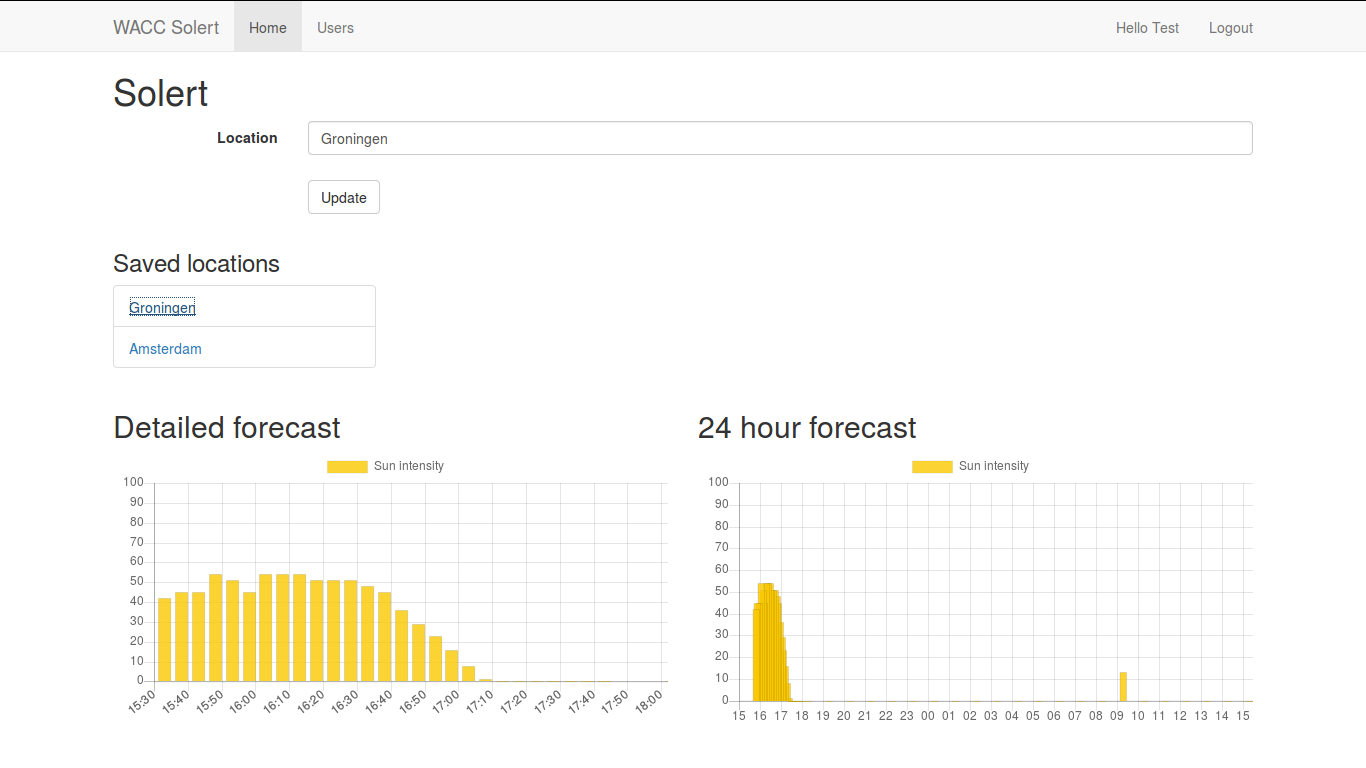
\includegraphics[width = \linewidth]{screenshot}
	\caption{Screenshot of the final web-frontend}
	\label{fig:screenshot}
\end{figure}

\section{Discussion}
In this part of the document we review and reflect on the project as a whole in a critical manner. A look is taken on docker swarm as a cluster orchestrator as well as the choice of databases.

\subsection{Docker Swarm}
Once you know how to use it, Docker swarm mode is a feature-rich tool for cluster orchestration. The inbuild service discovery, load balancing and fault tolerance suit many applications well. In detail we find Docker swarm mode to be very handy to set up stateless applications like our webserver or the crawler. On the other side setting up a stateful service like the databases, which bring their own implementations of cluster management is hardly combinable with Docker's concept of discarding crashed containers and starting new ones. Still, with some modifications it is possible.

The amount of programming that needs to be done to make Docker swarm mode capable of handling all our services is very low. Finding the right commands and parameters to configure Docker and the databases correctly takes most of the time as there are barely any tutorials or code examples online. The basic documentation of Docker swarm mode is available but is lacking in concrete examples. Furthermore it is difficult to find pages with information on Docker swarm mode, as you are likely to find pages referencing to the former cluster-management project of Docker, simply called Docker swarm.

In the end using Docker swarm mode was the right decision as it is easy to use in most cases and we expect the support to grow fast for more complicated cases. We think about publishing our work as there is no complete explanation on how to set up a Cassandra or MongoDB cluster using Docker swarm mode online yet.

\subsection{Scala}
Using Scala worked out well. After a difficult start of setting it up, get a basic demo working and getting a connection to a single database instance, it worked out fine. Since the programming language Scala was new to both of us, we had to put quite some effort into it to understand how it works.

The Play Framework provides a nice boilerplate to start a nice web application, although starting up the application after most code changes made development quite slow. However, we like that Scala compiles the code and knows at build time if the application can be run.

\subsection{Database}
In this project are two different databases integrated for the storage of data. This makes the application itself stateless, as all information is read from and written to the database. Therefore, the application can scale well in terms of the choice of the databases.

As the choice of Cassandra is well suited for the use-case of dealing with time based data, we feel very comfortable with this choice.

As for the choice of MongoDB for user management, it feels at this stage of the project over-engineered. In the beginning of the project we are using a very little amount of user data, but we see already the upcoming changes in the future development of the project. For these, the project is already ready and set up in a flexible way.

Luckily, both databases can work in a cluster mode out of the box with little, but at least for MongoDB, manual configuration. After the set-up period, the databases run and do not need any kind of maintenance.

\subsection{Future improvements}
Future improvements include our optional goals, which were not able to finish in the time of the project. This include the selection of a location via a Google Maps widget and also a general map view of the Netherlands with an overlay of the current sun shine situation.

Additionally, the application should also provide the functionality to request the current location of the user and query the sun shine data without typing in the current location first, but instead via the GPS coordinates provided by the smartphone or web browser.

Secondly, the front-end should push the sun shine data to the user directly, when new data is available. Currently the front-end always polls for new updates, but these calls can be reduced by a change in architectural design.

Thirdly, it would be an improvement to make more use of the features of docker swarm mode by distributing the services on more machines. Due to our limited hardware resources we were not able to run the application on more than three virtual machines.
%Thirdly, the options of docker swarm mode should get more explored. So far, most services run on all virtual machines, which the crawler being the exception with only a single instance. As the resources of the authors' computers are limited, the authors were unable to investigate this feature and separate the services more - although we believe it should work.

Furthermore, a future feature is a daily sun shine report via email. This would need another service to the application, but does not need a change in the current architecture.

%\bibliographystyle{alpha}
%\bibliography{sample}

\end{document}